\section{Financial Event Prediction}
%\KZ{I think you can combine sec 3 with sec 4 and just call it ``financial event prediction''. You should focus more on showing what the demo will achieve using an example and a screen shot of the demo, and lless about the internal archi or mechanism. This paper sounds too much like a tech paper now.}
Figure \ref{fig:causal_reasoning_architecture} sketches the WoLong system.
Given a sentence containing an event, WoLong will tell you the events this event will lead to (prediction) or the events that cause this event (explanation). 

\begin{figure}[htbp]
	\centering
	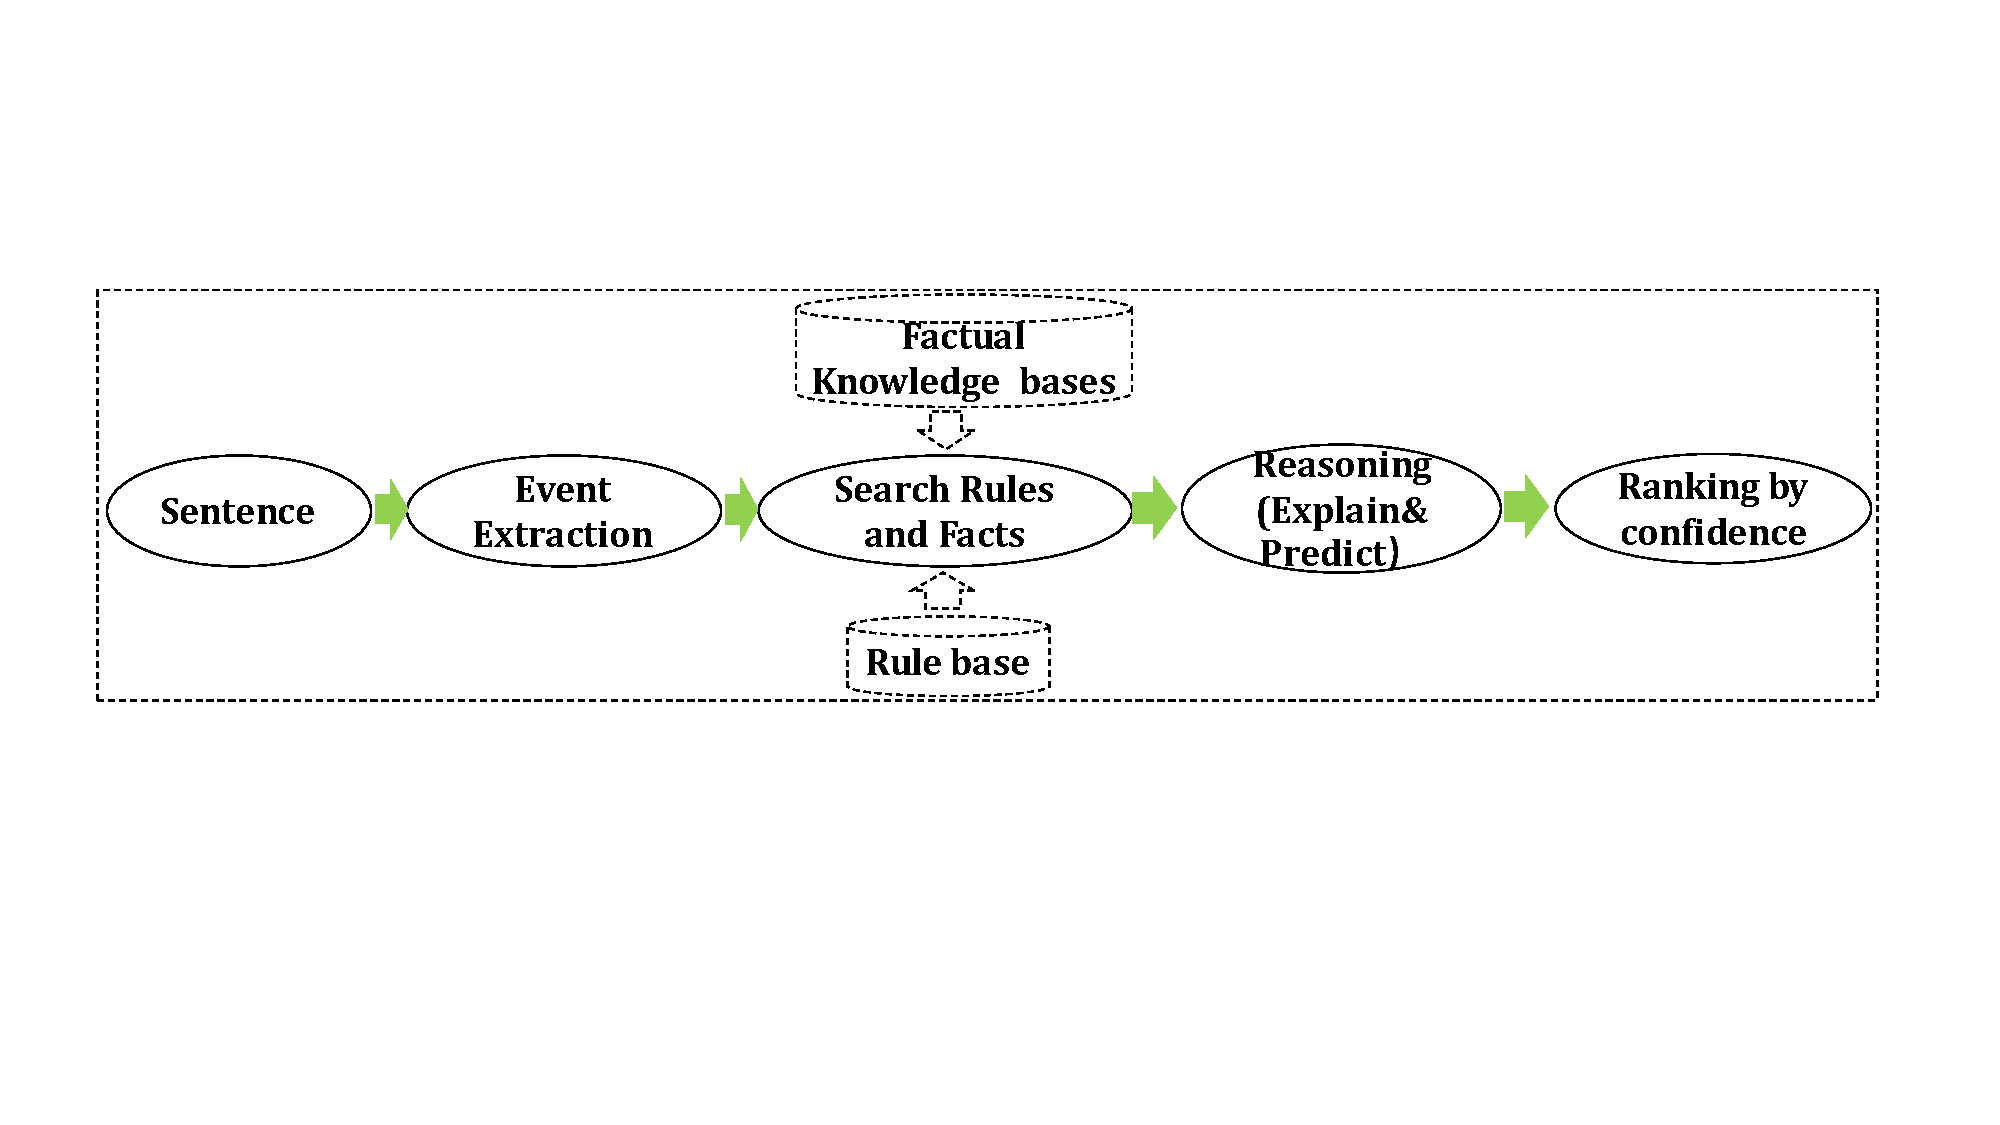
\includegraphics[width=0.95\columnwidth]{figures/causal_reasoning_architecture}
	\caption{WoLong System}
	\label{fig:causal_reasoning_architecture}
\end{figure}

\textbf{Event Extraction:} Given a Chinese sentence, typically a financial news title, parse it with Stanford CoreNLP tool\cite{Manning}, and extract the structured event with the quintuple format. 
\textbf{Search for Related Rules/Facts:} For this structured event, search for the related rules and facts in order to reduce inference time in Prolog. When searching for rules to predict (explain), specific event extracted from the input sentence matches the cause (effect) in the rule via Zh-Probase. For example, extracted specific event ``suffer(`',Thailand,earthquake,attack)" matches ``suffer(`',X,Y,attack)" in rule (1) by instantiating X to Thailand and Y to earthquake, which satisfies both isA(X,country) and isA(Y,disaster). In this way, we can acquire rule (1). Then, we use the depth-first search algorithm to search for other related rules based on rule (1). Last, we search for all facts used in these related rules from Zh-Probase and Zh-ConceptNet.
\textbf{Prolog Code Generation:}
We convert all retrieved human-readable rules and facts into standard Prolog code and also add some auxiliary code, see an example in Section \ref{sec:example}.
\textbf{Reasoning:}
To implement uncertain reasoning, we use multiplication to simulate the decline of the confidence in reasoning and set a threshold to prevent the Prolog from reasoning too deeply, which will lead to unreasonable predictions. Small modification of Prolog code 
is enough to reason with uncertainty, so we choose the mature and reliable SWI-Prolog\footnote{\url{http://www.swi-prolog.org/}} \cite{Wielemaker2010}, instead of ProbLog \cite{de2007problog} and PSL \cite{bach:jmlr17}.
\textbf{Ranking:}
Finally, it returns the top K events(event chains) sorted by the confidence (averaged) of the used rules.